\documentclass[tikz,border=3pt]{standalone}
\usepackage{lmodern}
\usepackage{amsmath}
\usetikzlibrary{positioning,calc,backgrounds,decorations.pathreplacing}

\definecolor{reportsage}{HTML}{344E41}
\definecolor{reportgrey}{HTML}{6B6B6B}
\definecolor{reportsagetint}{HTML}{E2EEE0}

\begin{document}
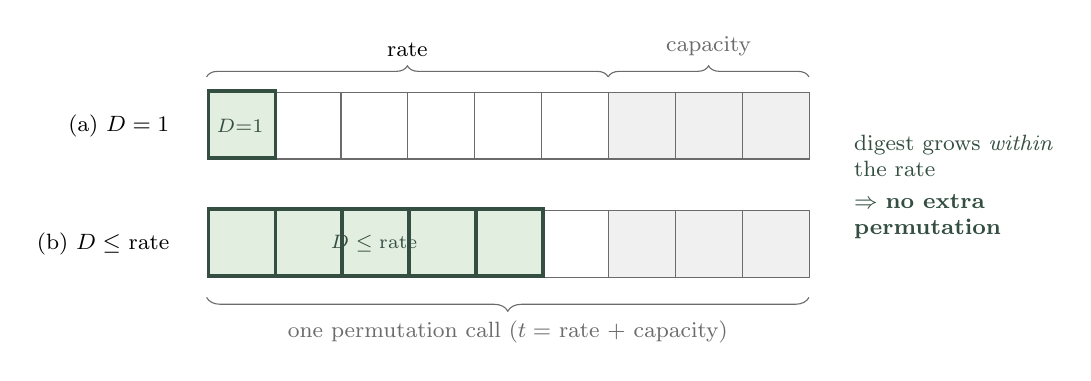
\begin{tikzpicture}[
  cell/.style={draw=reportgrey, minimum width=0.85cm, minimum height=0.85cm, anchor=south west},
  ratecell/.style={cell, fill=white},
  capcell/.style={cell, fill=black!6},
  digcell/.style={cell, fill=reportsagetint, draw=reportsage, very thick},
  lbl/.style={font=\footnotesize, text=reportgrey},
  font=\small,
]

% geometry
\def\w{0.85}        % cell width
\def\rate{6}        % rate cells
\def\cap{3}         % capacity cells
\pgfmathsetmacro{\total}{\rate+\cap}

% ---------- Case (a): D = 1 ----------
\def\ya{1.9}
% capacity (rightmost) and rate cells for row a
\foreach \i in {0,...,5} {
  \node[ratecell] at ({\i*\w},\ya) {};
}
\foreach \i in {6,7,8} {
  \node[capcell] at ({\i*\w},\ya) {};
}
% digest highlight: 1 rate cell
\node[digcell] at ({0*\w},\ya) {};
\node[font=\scriptsize, text=reportsage] at ({0*\w+0.5*\w},{\ya+0.43}) {$D{=}1$};

% case label
\node[lbl, anchor=east, text=black] at ({-0.35},{\ya+0.43}) {(a) $D=1$};

% ---------- Case (b): D = several ----------
\def\yb{0.4}
\foreach \i in {0,...,5} {
  \node[ratecell] at ({\i*\w},\yb) {};
}
\foreach \i in {6,7,8} {
  \node[capcell] at ({\i*\w},\yb) {};
}
% digest highlight: 5 rate cells (D <= rate)
\foreach \i in {0,...,4} {
  \node[digcell] at ({\i*\w},\yb) {};
}
\node[font=\scriptsize, text=reportsage] at ({2*\w+0.5*\w},{\yb+0.43}) {$D\le\text{rate}$};

\node[lbl, anchor=east, text=black] at ({-0.35},{\yb+0.43}) {(b) $D\le$ rate};

% ---------- region brackets / labels on top ----------
\def\ytop{2.95}
% rate brace
\draw[decorate, decoration={brace, amplitude=4pt}, reportgrey]
  ({0},\ytop) -- ({\rate*\w},\ytop)
  node[midway, above=4pt, lbl, text=black] {rate};
% capacity brace
\draw[decorate, decoration={brace, amplitude=4pt}, reportgrey]
  ({\rate*\w},\ytop) -- ({\total*\w},\ytop)
  node[midway, above=4pt, lbl] {capacity};

% ---------- "one permutation call" brace spanning full state, bottom ----------
\def\ybot{0.15}
\draw[decorate, decoration={brace, mirror, amplitude=5pt}, reportgrey]
  ({0},\ybot) -- ({\total*\w},\ybot)
  node[midway, below=5pt, lbl] {one permutation call ($t=$ rate $+$ capacity)};

% ---------- annotation note ----------
\node[align=left, font=\footnotesize, text=reportsage, anchor=west]
  at ({\total*\w+0.45},{1.55})
  {digest grows \emph{within}\\ the rate\\[2pt]
   $\Rightarrow$ \textbf{no extra}\\ \textbf{permutation}};

\end{tikzpicture}
\end{document}
